\subsection{Opret Bruger}
I dette afsnit vises design, bruger grænseflade, implementering og test for 'Opret Bruger' viewet. For den fulde dokumentation henvises til Arkitektur og Design dokumentationens afsnit \ref{Design-sec:Opretbruger}.
\subsubsection{Design}
Sekvensdiagrammet for 'Opret Bruger' viewet til Rambøll Tilsyn, kan ses på figur \ref{fig:OpretBrugerSekvens}. Figuren viser det logiske flow der sker når brugeren vil oprette en bruger.
\begin{figure}[H] % (alternativt [H])
	\centering
	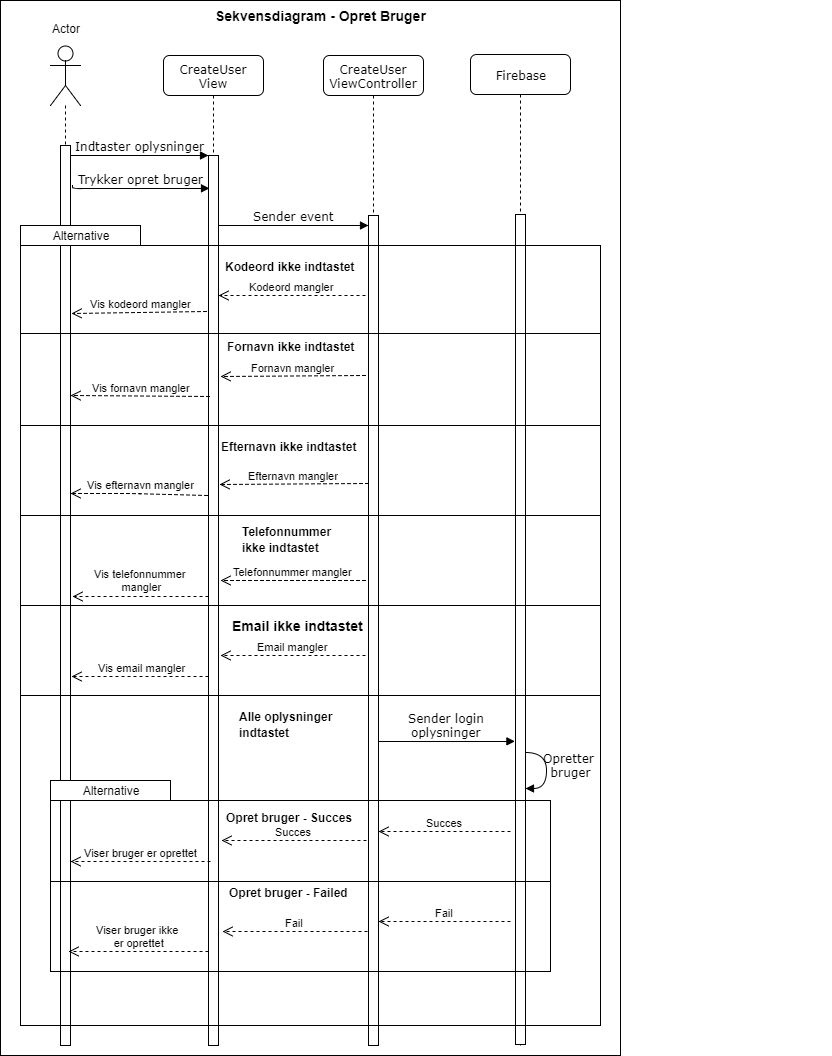
\includegraphics[height=18cm, width=15cm]{Design/Applikation/OpretBruger/OpretBrugerSekvensDiagram}
	\caption{Sekvensdiagram for Opret Bruger i Rambøll Tilsyn.}
	\label{fig:OpretBrugerSekvens}
\end{figure}

\subsubsection{Grafisk brugergrænseflade}
Den grafiske brugergrænseflade for 'Opret Bruger' viewet består af felter, så at bruger kan indtaste alt det information, der skal bruges når der skal oprettes en ny bruger. Se figur \ref{fig:OpretBrugerView}
\begin{figure}[H] % (alternativt [H])
	\centering
	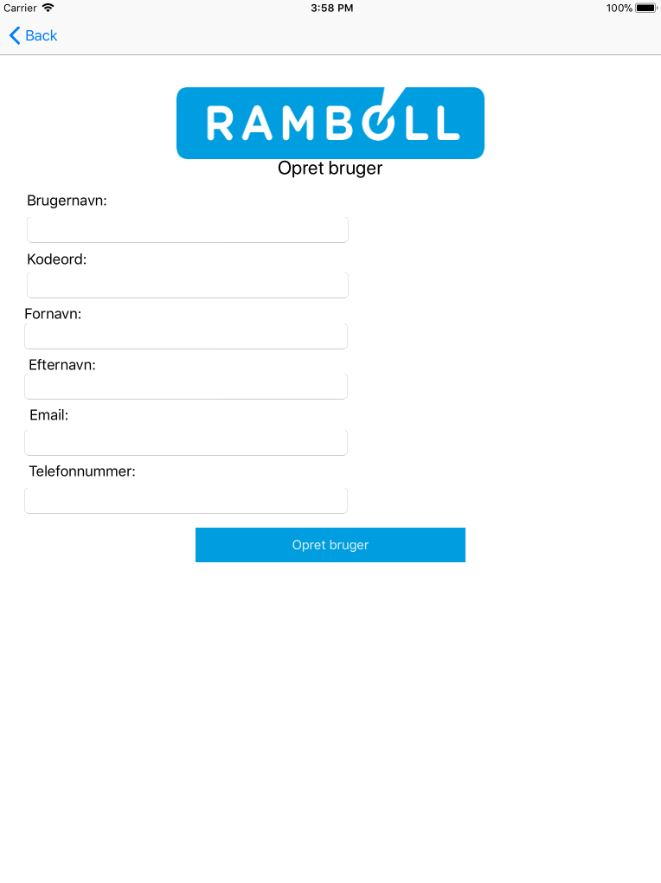
\includegraphics[height=12cm, width=10cm]{Design/Applikation/OpretBruger/OpretBrugerView}
	\caption{Opret bruger viewet som det er implementeret i Rambøll Tilsyn.}
	\label{fig:OpretBrugerView}
\end{figure}

\subsubsection{Implementering}

\subsubsection{Test}

\clearpage